% Play-and-judge evaluation (2D renderer).
% Source: docs/figures/judge2d.svg — edit that, then regenerate the PDF with
%   node scripts/render-figure.mjs docs/figures/judge2d.svg
%
% Drawn at 440pt wide so text stays legible at either venue's width:
%   NeurIPS: single column, \textwidth = 5.5in (396pt) -> scaled to 0.90
%   ICML:    two columns, use figure* at \textwidth = 6.75in (487pt) -> scaled to 1.11
% Do not set it at \columnwidth in a two-column template (~3.25in): the smallest text
% would fall to about 3.8pt.

% NeurIPS (single column)
\begin{figure}[t]
  \centering
  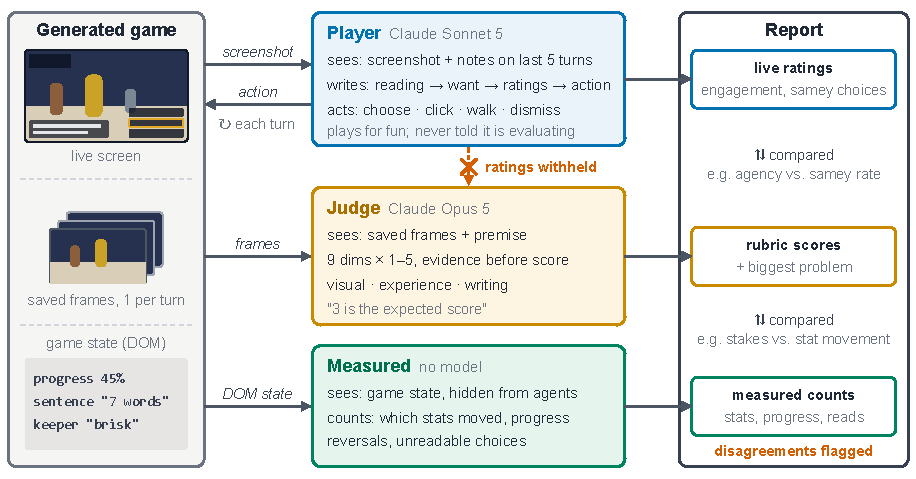
\includegraphics[width=\textwidth]{figures/judge2d.pdf}
  \caption{\textbf{Play-and-judge evaluation.}
    A \emph{player} agent (Claude Sonnet~5) plays the generated game in a headless
    browser from screenshots alone, carrying only its own notes on the last five turns,
    and records per-turn ratings before each action. Afterwards a separate \emph{judge}
    (Claude Opus~5) scores the saved decision frames---one per turn, plus the start and
    final screens---on nine 1--5 dimensions, writing its evidence before each score. The
    judge never sees the player's ratings, and neither agent sees the game state, which
    a model-free component reads directly from the DOM. The three signals are compared
    and disagreements are flagged: for example, a judge awarding \emph{stakes}~$\geq 4$
    when no tracked stat changed consistently.}
  \label{fig:play-and-judge}
\end{figure}

% ICML (two columns): same body, spanning both columns
% \begin{figure*}[t]
%   \centering
%   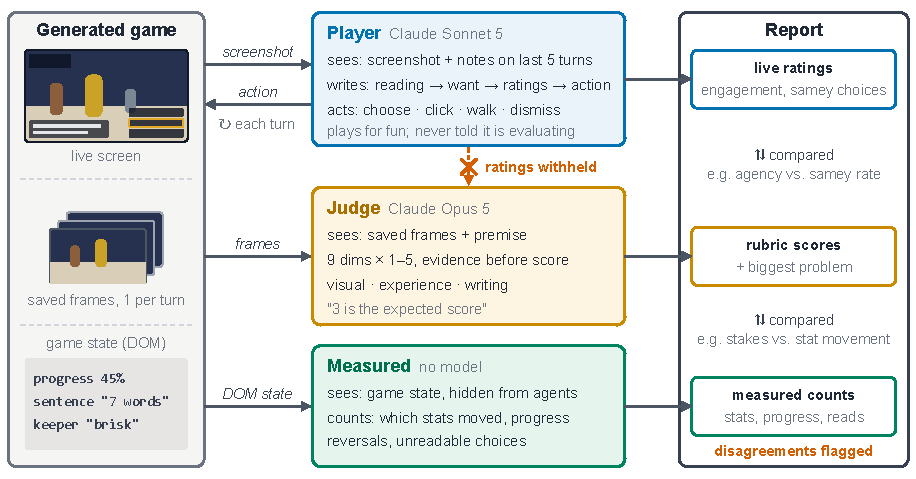
\includegraphics[width=\textwidth]{figures/judge2d.pdf}
%   \caption{...as above...}
%   \label{fig:play-and-judge}
% \end{figure*}
